\chapter{General overview}


\section{Current business pipelines}

It is very important to understand existing processes before attempting to automate these tasks. Atrato has partnered up with numerous merchants with possibly more than one store throughout Mexico. Every single partnership was discussed and agreed upon different terms, resulting in different expectations regarding how the money will be disbursed once a credit is granted through Atrato’s application process. These processes could either be monthly, weekly, daily, or individually per credit. Additionally, merchants could be conditioned to specific commissions depending on different factors like their monthly origination or if they were on a specific trial period. All these rules were not specifically written down nor followed any guideline. This meant that every time a disbursement needed to be made, the person in charge should review every commission agreed and compute the merchant’s monthly origination to know exactly what amount and in what conditions should the disbursement be made.

\subsection{Understanding Atrato’s Partners, Merchants and Stores}

Atrato’s partners are those commercial allies that offer its Buy Now Pay Later service as part of their payment options. These partners are internally classified as merchants and each of these merchants could have 1 or more registered stores.\\

The application process for a loan with Atrato takes place through Atrato’s web application by filling in information about the customer’s personal profile and financial information, indicating the merchant and store in which the loan will take place. Once the application is fully authorized by Atrato and the customer has finished the signature of its digital contract, then the store proceeds to deliver the product to the customer. Now, depending on the type of disbursement agreed upon the merchant’s registration, the money regarding the purchase will be transferred to the merchants banking account. This describes the process for a single application, but multiple applications need to be handled both by Atrato’s partners and Atrato’s internal team.

\subsection{Disbursement process}
The disbursement of a credit could be as simple as taking the amount of the credit and transfer it to the bank account related to the merchant. The complexity is added when a merchant does not want to receive plenty of bank transfers per day or even per week and rather have all the money disbursed as a single transaction at the end of the month. Since every partner expects this task to be handled upon their own agreed terms, every bank transfer needs to be carefully reviewed. Additionally, just like a partner can have their own terms, Atrato has its own specifications and requirements to every partner. Some commissions may be charged to the partner depending on their specific monthly origination and type of partnership. Furthermore, previously disbursed credits could be later cancelled or a change in amount may happen for many reasons, leading to a negative balance for the merchants.\\

Taking all these factors into consideration, the money disbursement is made firstly depending on the expected disbursement periodicity, then the total amount to be transferred is computed depending on the number of credits and their commission and this amount is manually sent in a single bank transfer.\\

Once the bank transfer is successfully confirmed, a report is generated indicating every credit that was part of the disbursement, their corresponding commission and any change in amount or cancellation that was taken into account to compute the total amount. This report is then sent to every single merchant providing complete transparency and understanding of every bank transfer that is sent.

\subsubsection{Partner’s dashboard}

Every partner has access to an internal dashboard where they can visualize and manage their customers’ applications and give follow ups on each product’s delivery or cancellation. The money regarding a new credit will not be disbursed until the partner notifies the delivery of the product through their dashboard. This notification works as Atrato’s triggering event to dispatch the money disbursement, the process that is intended to eventually be fully automated. This process is very important to be sure that no credit is disbursed before they are marked as \textit{delivered}. Once the credit’s product is delivered, the partner can visualize when the credit is disbursed. This dashboard is helpful to compare the information received from the disbursement’s report and what they visualize as the credits that were already delivered and disbursed.

\subsection{Compatibility with current business and application processes}
An active customer’s application turns into a Credit once the information is validated, every required document is uploaded and an offer is sent. If the customer agrees to the term’s presented in the offer, then it goes through a digital signature process, where all the details of the credit can be confirmed. Once the signature is generated, the Credit is finally created. It is in this moment where the calculations for the Credit’s commission need to be made to know exactly on what terms it was granted. The existing architecture supported a static commission per merchant, which was immediately assigned to the Credit, but not necessarily represented the correct commission.\\

A merchant’s commission could change every month depending on the previous month’s origination. Furthermore, depending on the type of merchant the commissions could vary even depending on the total number of payments agreed for the credit. Temporary promotions should also be considered in the process before deciding the exact commission for every credit, where a specific deal for interest free months for the end customer could represent a higher commission for the merchant offering this promotion.\\

All these factors must be considered before attempting to automate the disbursement process, without implying a change on current application or business processes.\\

Every agreed commission, trial period and origination thresholds for every merchant should be saved in a standardized manner, enabling a better understanding and implementation of the terms agreed.

\section{Automation of disbursement process requirements}
The first step towards this automation should be creating a detailed pipeline of the process. Every task and validation that was manually done before transferring a partner’s origination to their bank account will now need to be defined and structured in a regulated process.\\

The automation of such a delicate process can be achieved through the development of a modular balance system for each of Atrato’s partners. This balance system should be completely traceable, meaning that we should be able to know what is happening all the time, exactly how the computations are made and every factor that is affecting a partner’s balance. It should be able to be handled independently for each partner with the possibility to disable the automation for some of them at any moment. A security step should be implemented, where some balance systems could require a manual confirmation of the bank transfer before they are sent. This could be helpful for transitioning from a manual process with some partners into the whole automation pipeline. \\

Additionally, an integration with Banco de Mexico, the Mexican Banking System regulatory agency is needed to handle bank transfers properly. Since Atrato has not yet the technology to independently make bank transfers from one account to another this integration will be done through a third party that provides all access and security that is required.

\section{Balance system for partners}
This system should be modular enough to handle even different bank accounts per merchant. Since every merchant could have different stores, the modularity of the banking system will be done individually per every store.\\

The system will describe every update to the store’s balance, enabling a complete understanding of how any contribution to the balance was made or how it was adjusted. It will relate every credit generation or cancellation, every money disbursement or cancellation of previous disbursements, and every manual adjustment to the on-going bank transfers.\\

The balance system will be handled through Balance Update objects which will eventually generate Bank Transfer objects, all of which will be triggered by some specific requirements or events. In the following sections we will get a general overview of these models. 

\subsection{Balance Updates}
A Balance Update will be every movement, transaction, adjustment, or cancelation that directly affects the system’s balance. Balance Updates serve as the linking entity between a confirmed credit and a store’s balance considering the appropriate commission. Every Balance Update will contribute in a way to the general balance, recording the previous balance and the new balance after its contribution. In this way, to effectively know the system’s current balance it would be enough to inquire the last Balance Update.\\

Balance Updates can be created through the confirmation or cancellation of a new credit, through the confirmation of a successfully disbursed Bank Transfer or through the cancellation of a previously confirmed disbursement. Furthermore, a Balance Update could be generated manually by the treasury team whenever an adjustment to the balance is required. Balance Updates could have different specifications, expected behaviors or status updates depending on their type. These specifications will be furtherly discussed in Chapter 3.

\subsection{Bank Transfers} 
A Bank Transfer object will be the entity describing the money movements between Atrato’s bank account and every store’s bank account. Bank Transfers will only be generated through and composed by Balance Updates and their status will be directly related. Once the Bank Transfer is sent through the online banking system a new Balance Update will be generated indicating the money disbursement. In the case of a cancellation or rejection of this Bank Transfer, then the general store's balance should be adjusted indicating that the disbursement was cancelled.

\subsection{Triggers}
Atrato’s partners require specific disbursement processes, whether it is a daily, weekly, or monthly disbursement of the credits approved during this period or an immediate disbursement per credit. To allow this flexibility, the generation of a Bank Transfer will be initiated through specific triggers. Every store can have one of the following disbursement types: Instant, Hourly, Weekly or Daily.\\

These four disbursement types will be triggered accordingly through Cron Jobs. Once these events are triggered, all pending Balance Updates will be considered for generating a new Bank Transfer only if the store's actual balance is higher than the minimum amount required for a Bank Transfer. This threshold is defined to avoid sending Bank Transfers with a low amount of money, since every banking transaction also represents a cost for the company. There may be some edge cases where the total amount of the pending Balance Updates is even lower than \$0.00, this just means that for some reason the system’s balance is negative and no money will be disbursed until the balance becomes positive again through the origination of more approved credits or any further update to the store’s balance. Note that all these updates can only be done through Balance Update objects.

\subsection{Understanding the correct handling of partner’s commissions}

Every merchant, as well as every store, has a standard commission. All the business logic regarding the correct amount for these commissions should be handled independently to the automatic disbursement process. \\

Commissions can change dynamically depending on different factors, like special promotions, discounts or regarding the merchant’s monthly origination. All these processes and specifications should not interfere with the automatic disbursements. Every credit must have a commission assigned before it can be approved for disbursement. This will be the commission that will be considered for the computation of the amount for the Balance Update generated by the approval of a credit. \\

Independently of how a partner’s commissions vary, since the commission is directly assigned to the credit, these two business processes will not interfere with one another.

\section{Refactor and Changes}

Current business processes and the existing models for merchants, stores and all the structure for selecting a credit’s loan term where not able to support a new system where disbursements could be automated. Since the disbursement of a credit is the missing link that could complete the full automation of the credit application and lending process, all the entities involved converge in this point and some of them will require some very specific changes: A store’s bank account should be validated and ready to receive payments, a credit’s commission should be able to be determined according to the term selected, the amount requested and any applicable promotion that could be involved. Hence, additional to the changes in current pipelines are required and a complete re-design of the architecture related to how a customer could select the conditions of the loan they are applying to must be done.

\subsection{Registration of merchant’s pipeline changes}

During the registration process of any new merchant and their corresponding stores involved, the banking information of the stores should now be a required field. Once a merchant is added, its first store should be added as well, and every time a store is added its banking information should be included.\\

The treasury team oversees validating a merchant’s commission depending on the terms agreed upon their registration. To do this, a new attribute, \textit{isValidated}, will be added to both the Merchant and the Store models indicating if the information has already been validated by the treasury team or if it needs further validation. This extra step is now included as part of the registration process of a merchant. Every time the information of a merchant or a store is added or edited, the \textit{isValidated} flag will be set back to false, indicating that a new validation of the treasury team is needed.\\

The whole registration pipeline is mounted in a dashboard developed for internal use with CRUD operations. With any subtle change in the Update method, as shown in the code snippet below the \textit{isValidated}, the spread sintax is used to make this flag will always turn back to false when used, requiring an additional validation.

\begin{verbatim}
    await getRepository(Merchant).update(
        merchantId,
        {
         ...merchant,
         isValidated: false,
        }
       );
       
\end{verbatim}

A merchant cannot be validated if it does not have at least a validated store. Furthermore, any merchant that is not validated will not be displayed as an option in the application form.  Additionally, a new Model will be introduced: Payment Option. Its connection to the Merchant-Store model will be described in the following section.

\subsection{Refactor in partiality selection architecture}

During the development of Atrato’s customers’ application process the commissions for the merchants where not considered. Furthermore, with the iteration of commercial and partner acquisition processes, a credit’s commission became more complex. A credit’s commission can depend on the number of payments, the credit’s amount, and on-going promotions. To enable this dynamism a refactor of the internal architecture of the term selection options needed to be done.\\

Previously, whenever a merchant was incorporated to Atrato’s partners, a simple setup of the available terms was done. At this moment we only kept a record of the possible number of payments that were available for this merchant’s stores. Be it a range from 3 to 24 monthly payments. We needed to elaborate every merchant’s term options into a whole module of Payment Options, where every Payment Option includes specific interest rates depending on a customer’s risk profile, the number of payments, the requested amount and had expiring dates in order to work as promotions. In this way the Payment Options module could support the flexibility that was needed, and the availability of every option could be determined through a customer’s input.\\

This Payment Option model will refer to all the possible terms that a store could have and will include details regarding specific interest rates that could vary depending on a customer’s risk profile, and will include applicability filters for date and requested amount, the option to be tagged as a promotion, specifications on the specific merchant’s commission, a trial period specification and a flag indicating if its commission could be automatically updated to integrate with the on-going changes in a merchant’s commission due to their monthly origination. Please refer to Figure \ref{fig:uml_payment_options} for specific details on the model.\\

Payment Options will also go through the validation step from the Treasury team, following the same structure and process as before. Every Store should have at least a validated Payment Option before being completely validated. Now, the complete pipeline goes as follows:\\

Whenever a Merchant is added, its first Store should also be added, and the first payment option for the Store should be added as well. Regarding the validation process, it goes the other way around: Payment Options should first be validated before attempting to validate a Store, and once a Store is validated the Merchant can be validated as well. All of these works just as a general validation to make sure that there is no Merchant that does not have a valid Store and that every valid Store has at least a valid payment option.

\subsubsection{Diferences between Payments Per Store and Payment Options architecture}

\begin{figure} [H]
    \centering
    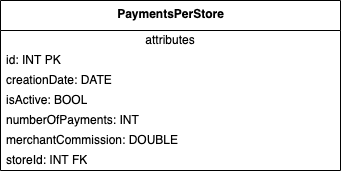
\includegraphics[scale = 0.6]{assets/uml/Payments_Per_Store.png}
    \caption{Payments Per Sotre UML}\label{fig:uml_payments_per_store}
\end{figure}

With the Payments Per Store Model a commission could directly be mapped to a specific number of payments, but there exists zero flexibility regarding a change of commission depending on the requested amount nor any distinction between a regular term or any offered promotion. Furthermore, interest rates need to be handled independently and could not directly be related to the number of payments that a customer selects.

\begin{figure} [H]
    \centering
    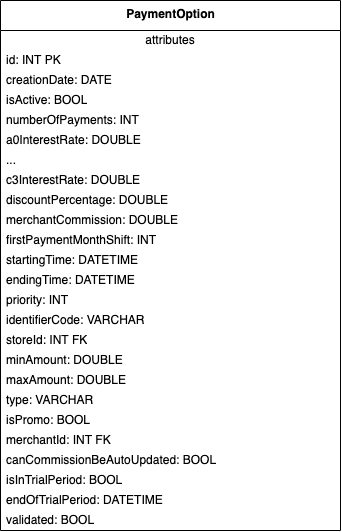
\includegraphics[scale = 0.6]{assets/uml/PaymentOptions.png}
    \caption{Payment Option UML}\label{fig:uml_payment_options}
\end{figure}

On the other side, with the Payment Option model, interest rates can be mapped directly to a customer's specific risk profile, ranging from A0 to C3; and every Payment Option includes filters to determine its elegibility based on the application's requested amount. Commissions can now be mapped and determined based on specific number of payments. Additionally, any promotion could just be directly represented as an additional Payment Option, and the priority of Payment Options with the same number of payments could be determined as well.\\ 


For new Merchants, a trial period can be determined and the Payment Options offered during this trial period could also integrate with this new model. By enabling this total flexibility in commissions and interest rates, added with the elegibility filters, every regular or specific Payment Option that Atrato wants to offer can now be mapped to the options that a Merchant can offer. These Payment Options can be either linked to only a specific Store or directly to a Merchant, indicating that all of the Stores of that Merchant in particular will have the Payment Option available.